\section{Hardening di base e controllo dell'accesso}

\subsection{Introduzione alla sicurezza}
Quando si parla di sicurezza, e' bene comprendere che quest'ultima non si realizza attraverso un particolare prodotto software o hardware acquistabile in mercato;
\begin{center}
	``La sicurezza e' il risultato di un \textbf{processo}"
\end{center}
Bisogna infatti pensare alla sicurezza come al risultato di un processo che prende in considerazione non solo tutti gli aspetti tecnologici ma anche quelli umani. Ottenere un livello accettabile di sicurezza richiede pazienza, attenzione, conoscenza e determinazione. Vediamo qualche principio generale da tenere in considerazione:
\begin{itemize}
	\item Uno dei pochi punti fermi a tal proposito e' che la sicurezza si gestisce efficacemente solo vietando qualsiasi comportamento non esplicitamente consentito. Allo stesso tempo. cio' che e' consentito deve essere svolto con i diritti piu' restrittivi e compatibili con l'esecuzione del compito.
	\item La sicurezza e' antagonista dell'usabilita': e' necessario cercare soluzioni che pongano meno ostacoli possibili fra il servizio che si vuole garantire in maniera sicura e gli utenti finali che voglioni utilizzarlo.
\end{itemize}
Il campo della sicurezza informatica e' molto ampio, ma viene generalmente discusso in rapporto a tre parametri fondamentali, che rientrano sotto l'acronimo di ``\textbf{CIA triad}":
\begin{center}
	\item Confidentiality (Riservatezza)
	\item Integrity (Integrita')
	\item Availability (Disponibilita')
\end{center}

\paragraph{Confidentiality} 
La confidenzialita' tratta la \emph{riservatezza} dei dati. L'accesso alle informazioni deve essere limitato ai soggetti autorizzati. Autenticazione, controllo degli accessi e cifratura delle informazioni sono alcuni sottocomponenti che contribuiscono ad assicurare questa proprieta'.

\paragraph{Integrity}
L'integrita' rappresenta l'\emph{autenticita'} delle informazioni. Le tecnologie volte a determinare l'integrita' dei dati garantiscono che questi siano validi e non siano stati alterati in maniera non autorizzata. Affronta anche l'affidabilita' delle fonti di informazione. Quando un sito web sicuro presenta un certificato TLS firmato, garantisce all'utente non solo che le informazioni che vengono scambiate sono protette da meccanismi crittografici ma anche che un'autorita di certificazione (\emph{CA, Certification Authority}) ha verificato l'identita' della sorgente.

\paragraph{Availability}
La disponbilita' esprime l'idea che le informazioni debbano essere accessibili da soggetti autorizzati in qualsiasi momento questi ne abbiano necessita'. Altrimenti, le informazioni non avrebbero valore.
\\\\
I principi della CIA Triad ci danno una linea guida per progettare, implementare e mantenere i sistemi e le reti,
attraverso un approccio solido e sistematico.
\subsubsection{Compromissione della sicurezza}
In questa sezione diamo un occhiata generale a quali sono i problemi legati alla sicurezza nel mondo reale. Gran parte delle modalita' con le quali e' possibile compromettere un sistema rientrano nelle seguenti categorie.

\paragraph{Social Engineering}
L'essere umano, utente (e amministratore) di un sistema e' l'anello piu' debole nella catena di sicurezza. Nessun tipo di tecnologia puo' proteggere dall'elemento umano - bisogna ssicurarsi che la propria comunita' di utenti sia fortemente sensibilizzata e abbia una grande consapevolezza delle problematiche e delle minacce legate alla sicurezza cosi' che possano diventare anch'essi parte della difesa.

\paragraph{Software Vulnerabilities}
Negli anni, sono stati scoperti una quantita' innumerevole di falle di sicurezza all'interno del software di uso comune e non. Gli hacker si sono resi abili nello sfruttarle a loro vantaggio, manipolando e compromettendo interi sistemi. In un certo senso, i sistemi di sicurezza open source hanno un vataggio in termini di sicurezza. Il codice sorgente di Linux e FreeBSD e' messo a disposizione di chiunque, e migliaia di persone possono mettersi in gioco e analizzare ogni singola riga di codice alla ricerca di un'eventuale crepa da sfruttare. Si pensa quindi che questo approccio porti ad ottenere migliori risultati in termini di sicurezza e affdabilita' del software di contro a sistemi operativi proprietari (e quindi con codici sorgenti privati), ai quali e' concesso l'accesso soltanto ad un numero limitato di persone.

\paragraph{Distributed denial-of-service attacks (DDosS)}
Un attacco di tipo DDoS punta ad interrompere o impattare negativamente le performance di un servizio, compromettendone la disponibilita' agli utenti legittimi. Questi si realizzano spesso attraverso la saturazione del traffico di rete , inondando di richieste un determinato servizio cosi' da saturare le risorse disponibili. Spesso per condurre un attacco di questo tipo gli Hacker si appoggiano a ``\emph{botnet}", ovvero intere reti di dispositivi compromessi e controllati da remoto a fini malevoli. Gran parte della responsabilita' legata alla prevenzioni di questi attacchi ricade su chi gestisce la rete. Esistono software e componenti hardware appositamente progettate per rilevare attacchi di questo tipo e contrastarli continuando a garantire la disponibilita' del servizio. Ad ogni modo queste tecnologie non sempre riescono a mitigare perfettamente questi attacchi e le minacce sono in continua evoluzione.

\paragraph{Insider abuse}
Dipendenti, terzisti e consulenti sono agenti fidati di un'organizzazione ai queli spesso vengono garantiti privilegi speciali. Spesso pero' questi privilegi vengono abusati. Interni possono rubare o rivelare informazioni, corrompere sistemi sotto pagamento, o devastare per motivi politici. Queste tipologie di attacchi sono spesso i piu' complessi da rilevare per questo motivo solo le organizzazioni piu' rigorose controllano sistematicamente i loro dipendenti.

\paragraph{Network, system, or application configuration errors}
Il software puo' essere configurato in maniera sicura o non tanto sicura. Questo viene sviluppato per essere utile e non noioso, di conseguenza spesso l'opzione ``non tanto sicura" e' quella standard. Gli hacker spesso si garantiscono l'accesso ai sistemi passando per feature considerate utili e convenienti in circostanze meno insidiose: account senza password, firewall con regole molto permissive, database non protetti, etc. Un tipico esempio di una vulnerabilita' e' la pratica standard di concedere ad un sistema linux di fare boot senza che il boot-loader richieda alcuna password. Questa mancanza apre le porte ad attacchi fisici. Comunque, e' un esempio perfetto della necessita' di trovare un equilibrio fra sicurezza e usabilita'. Richiedere una password significa impedire , in caso di reboot del sistema, il completo restart della macchina , richiedendo quindi la presenza fisica di un amministratore di sistema.

\subsubsection{Messa in sicurezza fisica}
La predisposizione fisica di un sistema ha un'\textbf{importanza rilevante}. Un server e' prima di tutto un sistema di calcolo, collocato in un ambiente e connesso a una varieta' di dispositivi. Normalmente si tende a concentrare le difese sul fronte degli attacchi via rete, a componenti software come applicazioni e sistema operativo, ma tutte queste contromisure possono essere facilmente aggirate se si possiede accesso fisico al sistema. Le minacce principali in questione sono:
\begin{itemize}
	\item Furto dello storage o dell'intero calcolatore
	\item Connessione di sistemi di raccolta dati alle interfacce
	\item Avvio del sistema con un sistema operativo arbitrario
\end{itemize}
La gravita' di queste minacce dipende fortemente dallo specifico ambiente. Molti di questi problemi non si presentano piu' nello scenario comune che tende sempre piu' ad affidarsi a sistemi di virtualizzazione su Cloud gestiti esternamente, ma altri concettualmente simili sono appparsi, e la logica delle stesse contromisure si puo' adattare.
		
\subsection{Pianificare l'installazione del Sistema Operativo}
Introdotte le motivazioni per cui anche la predisposizione fisica gioca un ruolo importante nel processo di messa in sicurezza di un sistema, passiamo ora allo step successivo in un ipotetico ciclo di vita di un sistema. Dopo aver messo in piedi un hardware funzionante si procede con l'istallazione di un \textbf{sistema operativo}. 

\paragraph{Distribuzione}
Sempre per attenerci al principio del \emph{minimo privilegio} ossia non mettere in piedi niente che non sia strettamente necessario, cosi' da evitare a prescindere che venga utilizzato, il sistema che si vuole impiegare in questi casi e' un sistema ``ridotto all'osso", ovvero con la minima quantita' di utility e software essenziali al lavoro che la nostra macchina dovra' poi svolgere. Questa filosofia non si rispecchia molto nelle distribuzione che troviamo normalmente in circolazione che spesso , insieme all'installazione del sistema operativo, comprendono un set di programmi e di utility molto vasto per venire in contro a quelle che potrebbero essere le varie esigenze di un utente finale. In ambito aziendale il discorso diventa piu' complesso, in particolar modo per quanto riguarda i sistemi operativi: se si necessita di un supporto commerciale alla distribuzione linux che si intende impiegare si puo' scegliere solo fra un gruppo ristretto di alternative (\emph{Red Hat, Canonical, SUSE}), dipendendo da quelle che saranno poi le distribuzioni messe a disposizione del cliente cosi' come sono state certificate dal fornitore , per poi accordare direttamente con quest'ultimo cosa quali componenti sono essenziali e quali invece si possono togliere per arrivare a rispecchiare le nostre esigenze.

\subsubsection{Organizzare dati e software}
Un altro aspetto sicuramente di notevole importanza , in particolare orientato ad un discorso di scalabilita' e sicurezza, e' l'organizzazione dello spazio di memorizzazione. Il concetto di partizionamento di un dispositivo di memorizzazione la fa da padrone. 
\\\\
Storicamente si tendeva a partizionare varie aree dello stesso sistema (filesystem), in base alla loro funzione, su piu' filesystem e relativi dispositivi di memorizzazione in quanto le probabilita' che un disco potesse essere soggetto a guasti erano significative. In questa maniera si cercava di limitare il danno ad una singola porzione del sistema, garantendo che le altre , in particolare quelle contenenti i file di boot e configurazione di sistema , rimanessero accessibili e quindi fosse possibile comunque far partire le opportune procedure di ripristino e salvare quel che non e' stato soggetto a guasti (a patto che non fossero proprio queste ultime a corrompersi). Al giorno d'oggi questo criterio continua ad avere una sua validita' in particolare per limitare danni dovuti alla saturazione delle risorse. Se infatti si vanno a collocare in contenitori rigidamente separati dati di tipologie diverse (\emph{Dati critici per il sistema, dati utenti, dati temporanei, etc}) il fatto che una di queste partizioni sia suscettibile ad eventuali DoS o saturazione delle risorse non va ad influenzare la disponibilita' di altre funzionalita' del sistema. Questo d'altro canto risultava essere anche un lavoro molto complesso e delicato per il sistemista che doveva configurare i dischi, ovvero scegliere con cura come disporre le diverse partizioni su un hardisk, in quanto poi cambiarle risultava praticamente impossibile. 
\\\\
Fortunatamente questo tipo di limitazioni sono state oggi superate anche grazie a sistemi come \textbf{LVM} (\emph{Logical Volume Manager}) che permettono di gestire lo spazio in maniera totalmente flessibile. E' sempre importante notare pero', come l'introduzione di layer nuovi che quindi apportano ulteriori elementi di complessita non sia mai gratis; si ha infatti un impatto sulle prestazioni , che nel caso di LVM e' sostanzialmente trascurabile, ma anche un impatto sulla robustezza, dovuta al fatto che ogni qual volta si va a complicare un meccanismo, la probabilita' che uno degli ingranaggi che lo compone si inceppi aumenta proporzionalmente al numero di ingranaggi introdotti. All'opposto, quindi se voglio evitare di apportare complessita', ci sono anche soluzioni molto rigide: ad esempio posso configurare i miei sistemi in maniera tale che i dati veramente critici siano su dispositivi di sola lettura e che quindi siano resi sostanzialmente del tutto inalterabili.

\subsubsection{Partizionamento}
Un disco puo' essere visto banalmente con una stringa lunga di byte, essendo questi molto grandi, indirizzare il singolo byte sarebbe totalmente inutile, si tende racchiundere questi byte all'interno di \textbf{blocchi} numerati di dimensione fissa, generalmente blocchi da 4096 Byte (4KB). 
Possiamo quindi di fatto definire un disco come una sequenza di blocchi numerati. Dentro una di queste sequenze di blocchi numerati , ovvero dentro quello che chiamiamo un \textbf{block device} (\emph{dispositivo a blocchi}) e' possibile creare un \textbf{filesystem} attraverso un'operazione di \emph{formattazione}. 

\paragraph{Filesystem}
Possiamo pensare al filesystem come ad una struttura e un insieme di regole logiche per manipolare e organizzare in un albero gerarchico di diverse cartelle gruppi di dati (files) con la possibilita' di fare riferimento a questi attraverso dei nomi simbolici. Questa possibilita' viene concretizzata attraverso una mappatura tra nome logico e posizione fisica del dato associato. Tutti i filesystem hanno una caratteristica, cioe' danno per scontato che il contenitore (block device) che hanno a disposizione da organizzare sia privo di buchi, ovvero una sequenza di blocchi contingua. Sulla base di questa ipotesi e' possibile suddividere il block device in una serie di sotto-contenitori che dal punto di vista astratto risultano essere dei veri e propri dischi indipendenti.
\\\\
Il \textbf{processo di partizionamento} consiste quindi nel partire da un dispositivo a blocchi che ci mette a disposizione un elenco di blocchi disponibili, fisici, e nel suddividerlo in sottoinsiemi \textbf{contigui} di blocchi all'interno di ognuno dei quali vige una numerazione locale. Questa viene realizzata semplicemente attraverso una tabella che associa ad ogni partizione un identificativo (numero ordinale), il range di blocchi allocato (blocco di partenza e fine) e la tipologia della partizione, ovvero un'etichetta che ha prettamente un uso orientativo. 
Ogni partizione ``vive" in un mondo logico totalmente separato dalle altre. Questo significa che quando vado a formattare una di queste partizioni, posso creare filesystem di tipologie totalmente diverse, all'interno delle quali l'organizzazione dei dati non influisce su quella delle altre. Ogni partizione ha una sua dimensione massima che non puo' essere ecceduta dal filesystem. Nel caso abbia creato due partizioni distinte una per i dati utente e una per i file di sistema, la saturazione della prima non impedisce il corretto funzionamento del sistema, ma impedira' agli utenti di allocare nuova memoria per nuovi file.
\begin{wrapfigure}{R}{6cm}
	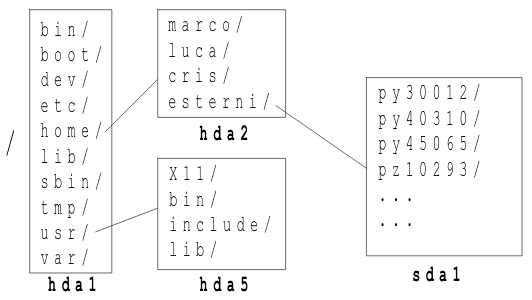
\includegraphics[scale=0.5]{"img/partitioning.png"}
	\caption{Lo schema in figura rappresenta la partizione:
		\\\\
		\begin{tabular}{ll}
			\textbf{Partizione} & \textbf{Mount point} \\
			\texttt{/dev/hda1} & \texttt{/}\\
			\texttt{/dev/hda2} & \texttt{/home/}\\
			\texttt{/dev/hda5} & \texttt{/usr/}\\
			\texttt{/dev/sda1} & \texttt{/home/esterni/}
		\end{tabular}}
\end{wrapfigure}
\paragraph{Linux} 
Linux identifica le partizioni attraverso dei file speciali con del tipo \texttt{/dev/sd*}. I file in \textbf{\texttt{/dev/}} sono \emph{block special} o \emph{character special}, cioe' non sono file che contengono dati, ma punti di accesso ai divice driver del sistema operativo, in particolare i primi adatti per l'accesso a blocchi di dati su dispositivi buffered (come appunto i dischi), i secondi per l'accesso a carattere a dispositivi come le porte ed i serial-bus. Oltre ai dispositivi fisici, un block device puo' rappresentare il punto d'accesso ance a dispositivi logici che si comportano allo stesso modo, ad esempio volumi RAID, LVM o di rete.
Ogni volta che creo un filesystem all'interno di una partizione, nella gerarchia complessiva del filesystem UNIX dovro' scegliere un \emph{mountpoint}, ovvero un punto di montaggio, che rappresentera' poi la mia via d'accesso verso quest'ultimo. 
\\\\
\paragraph{Filesystem Hierarchy Standard, FHS}
E' uno standard che definisce la struttura delle directory e relativo contenuto nei filesystem UNIX allo scopo di rendere piu' facili a programmi automatici ed utenti l'individuazione delle risorse, rendere piu' efficiente la condivisione di parti del filesystem e rendere piu' sicura la memorizzazione dei dati.
Le distinzioni di base che gidano alla corretta collozione dei dati in FHS sono 2:
\\
\begin{center}
\begin{tabular}{|l|l|l|}
	\hline
	& Condivisibili & Non condivisibili \\\hline
	Statici & es. \texttt{/usr} \texttt{/opt} & es. \texttt{/etc} \texttt{/boot} \\\hline
	Variabili & es. \texttt{/var/mail} \texttt{/var/spool/news} & es. \texttt{/var/run} \texttt{/var/lock} \\\hline
\end{tabular}
\end{center}
\\
\paragraph{Approfondimenti} Sezione \ref{filesystem}.


\subsubsection{Booting}
Una volta pianificata con attenzione la collocazione dell'hardware e la disposizione delle risorse, completiamo l'istallazione del sistema operativo e procediamo verso un primo avvio completo del sistema. Questa procedura attraversa \textbf{4 macro fasi} fondamentali:

\begin{figure}[H]
	\centering
	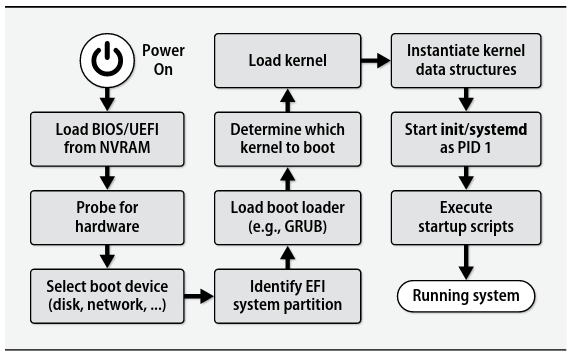
\includegraphics[scale=1]{img/linuxunixbootprocess.png}
	\caption{Linux and UNIX boot process}
\end{figure}

\paragraph{First-stage (Finding, loading, and running bootstrapping code)}
Sulla mainboard deel nostro sistema e' installata una memoria non volatile read-only (EPROM, flash*) all'interno della quale e' presente del codice, anche detto (\textbf{firmware}), tradizionalmente noto come \textbf{BIOS} (\emph{Basic Input Output System}), oggi ormai superato da un nuovo standard: \textbf{UEFI} (\emph{Unified Exstensible Firmware Interface}). 
\\
Il firmware, prodotto e preinstallato direttamente dal costruttore della scheda, e' in grado di agire a livello macchina consentendo di fare un inventario e configurare i dispositivi hardware installati sul sistema (\emph{Controller SATA, interfacce di rete, controller USB, sensori di potenza e temperatura}), potendo inoltre decidere se esporli, disabilitarli o nasconderli al sistema operativo. Consente inoltre di individuare da quali di questi possa eventualmente essere caricato ulteriore software, fare degli health-check per verificarne il corretto funzionamento, scegliere (attraverso un ordine configurabile) quale e' piu' opportuno e mandare in esecuzione lo step sucessivo.
Il BIOS si articola in due parti principali memorizzate entrambe in memorie non volatili, una che il vero e proprio firmware e l'altra si compone di tutta una serie di parametri di configurazione modificabili dall'amministratore di sistema attraverso un'interfaccia alla quale si accede premendo una combinazioni di tasti che varia in base al produttore e al modello dell' hardware (\texttt{F2, F8, F12}).

\paragraph{Second-stage (Finding,loading, and running the OS kernel)}
Il secondo step, nella procedura di avviamento del sistema, passa attraverso una seconda componente software, distinta da entrambi BIOS/UEFI e kernel del sistema operativo, che prende il nome di \textbf{Boot Loader}. Il compito principale di questo e' identificare e caricare il kernel appropriato del sistema operativo. Molti questi presentano anche un'interfaccia utente a boot-time che permette di selezionare, fra quelli presenti sul sistema, quale dei kernel o sistemi operativi mettere in esecuzione. Il fatto che questo sia un componente separato dal BIOS/UEFI e' dato dalla quantita' e varieta' di parametri necessarie a gestire e configurare l'avvio di un sistema operativo; sarebbe infatti impensabile inserire la ``consapevolezza" di tutti questi parametri e l'intelligenza per sceglierli correttamente all'interno BIOS che e' software che viene inserito in una mainboard lato produzione e mai piu' aggiornato per svariati anni essendo questo un elemento critico per la stabilita' del sistema, che contiene quindi solo gli elementi essenziali al funzionamento/interazione con la componente hardware del sistema.

\paragraph{Third-stage (Running startup scripts and system deamons)}
Una volta caricato il kernel ed eseguite le routine di inizializzazione, quest'ultimo avvia un serie di processi complementari ``spontanei" (in quanto avviati autonomamente dal kernel). Gran parte di questi sono parte dell'implementazione stessa del kernel e non per forza trovano corrispondenza in file all'interno del filesystem;e' possibile riconoscerli attraverso il comando \texttt{ps aux} da loro \texttt{PID} basso e le parentesi \texttt{[process-name]} attorno al nome del processo.
\\
Il kernel e' di per se un processo vero e proprio, con la caratteristica che essendo il primo processo ad essere effettivamente eseguito, quando il processore e' ancora in \emph{kernel-mode}, prende completo possesso del sistema e puo' procedere al caricamento dei vari device driver etc\dots creando quell'ambiente all'interno del quale e' poi possibile lanciare processi con privilegi fisici limitati (\emph{user-mode}). Il demone di amminsitrazione di sistema (\emph{system management deamon}), prende generalmente il nome di \textbf{init} e ha \textbf{process ID 1}. Il sistema concede ad \emph{init} un paio di privilegi speciali, ma per la restante parte e' un programma a livello utente esattamente come qualsiasi altro demone.

\newpage
\paragraph{Fourth-stage (Maintaining process hygiene and managing system state transitions)}
A questo step la macchina e il sistema operativo sono configurati. Il processi init si occupera' di gestire i \emph{runlevel} e i \emph{target} per coordinare l'inizializzazione del sistema, ovvero avviare i servizi nell'ordine corretto. Fara' quindi partire tutte le varie utility messe a disposizione dello user per iniziare ad utilizzare il sistema, ad esempio: il processo di \texttt{login} , eventuali ambienti grafici, etc\dots



\subsubsection{Sicurezza}
Ognuno di questi passi, dell'ottica di voler rendere sicuro il sistema, puo' essere protetto:
posso infatti stabile quali di questi step possano essere eseguiti autonomamente e quali invece richiedano l'inserimento di credenziali di autorizzazione per poter deviare dall'ordine predefinito delle cose. Il BIOS , ad esempio, puo' essere protetto da password, prestando attenzione al fatto che esistono dei meccanismi di reset in grado di ripristinarle a valori di default (purche' si abbia accesso fisico alla macchina). Lo stesso vale per il Boot Loader, e' possibile proteggere quest'ultimo con delle password. E' bene notare che questi meccanismi creano dei possibili problemi di disponibilita' non indifferenti, in quanto ad ogni riavvio (volontario o non) del sistema e' necessaria la presenza di un amministratore perche' quest'ultimo possa completare la procedura inserendo le varie credenziali. Per facilitare questo meccanismo, e' possibile impostare BIOS e Boot Loader in modo che richiedano delle credenziali solo nell'eventualita' in cui il processo di boot venga modificato rispetto a quello standard stabilito.
Sempre in termini di sicurezza, occurre notare che svariati sistemi operativi offrono una modalita' di esecuzione particolare (\emph{maintenance mode}) pensata per fare recovery in situazioni critiche, che al contempo e' possibile sfruttare per ottenere privilegi elevati all'interno di un sistema.
\\
\paragraph{Affidabilita' del software}
A questo punto dovremmo aver garantito nel percorso che va dall'accensione attraverso il pulsante \emph{power-on} al caricamento del sistema operativo, venga rispettata una sequenza prestabilita , ma non abbiamo preso in considerazione l'aspetto che concerne l'integrita', l'autenticita' e quindi l'affidabilita' del software che stiamo avviando. Partendo dall'alto, per quanto riguarda la sicurezza dei programmi che eseguiamo quotidianamente ci si affida generalmente ad un \textbf{Antivirus} o anti-malware di vario genere che hanno il compito di verificare l'integrita' delle applicazioni. A questo punto pero, bisogna considerato che l'antimalware e' un software che risiede un un disco fisico e che quindi per natura e' strutturalmente modificabile, 
\begin{center}
	\emph{chi verifica allora che questo stia effettivamente eseguendo il proprio compito o non sia stato modificato per tacere di fronte a comportamenti anomali?} \\
	Lo verifica chi lo installa e lo esegue, ovvero il \textbf{sistema operativo}. 
\end{center}
Se avessi a disposizione un sistema operativo \emph{trusted}, allora potrei quasi considerare inutile l'antimalware, ma non e' questo il caso. L'unico modo che abbiamo per avere una visione completa del sistema e' chiedere al sistema operativo, ovvero la nostra interfaccia a tutte le funzionalita' e l'hardware messo a disposizione dalla macchina. Se quest'ultimo fosse anch'esso danneggiato o compromesso, la visione di cio' che realmente sta accadendo sarebbe irrimediabilmente falsata. Abbiamo quindi la necessita' che il sistema operativo sia integro, autentico e affidabile. 
\begin{center}
	\emph{Chi verifica quindi che il sistema operativo che stiamo mettendo in esecuzione sia affidabile?}
\end{center}
Potrebbe farlo il Boot Loader, ma a questo punto ritorneremmo punto a capo, non potendo garantire che anche quest'ultimo non sia effettivamente stato corrotto. Lo stesso discorso, con tutte le complicazione tecniche del caso, vale per il BIOS.

\paragraph{Chain of trust}
L'unica cosa a cui effettivamente possiamo agganciarci per essere certi che non siano state fatte delle modifiche non autorizzate a tutta questa catena che parte dal bios fino alle applicazioni e' un dato che sia fisicamente \textbf{inalterabile}; cio' non puo' essere fatto a partire da un dato che e' scritto in un dispositivo, ad esempio un disco, che per sua natura e' fisicamente modifibile. Serve una quindi una \textbf{root of trust} (\emph{radice di fiducia}) aggianciata all'hardware: qualcosa di fisico che non possa essere \textbf{mai modificato} e al contempo possa essere \textbf{verificato}, e mi permetta di avviare una \textbf{catena di fiducia}. Se io so che il primo step dei 4, e' verificato partendo da un termine di paragone inalterabile, assolutamente affidabile, allora e' possibile propagare gli eventuali controlli di autenticita' ed integrita' su tutta la catena.

\subsubsection{Paradigmi di trusted boot}
Questa catena di fiducia nei sistemi moderni puo' essere implementata secondo due paradigmi diversi:

\begin{wrapfigure}{R}{6cm}
	\centering
	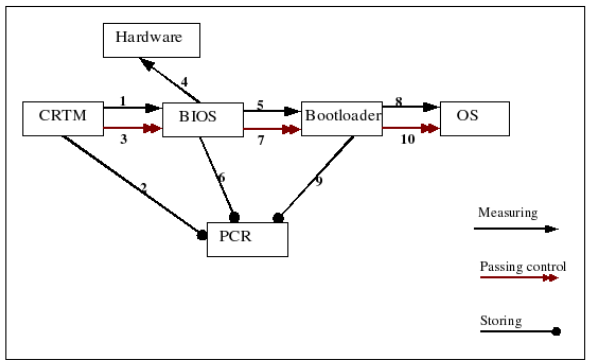
\includegraphics[scale=0.5]{img/trustedboot.png}
\end{wrapfigure}
\paragraph{Trusted Boot}\\
Questa si appoggia ad un co-processore crittografico (\emph{\textbf{TPM},Trusted Platform Module}) collocato sulla mainboard, con funzionalita' crittografiche e in grado quindi di verificare autenticita' e integrita', grazie anche a dati segreti ed immutabili contenuti internamente. In questo modo si evita di dipendere gia' dalla fase iniziale di software particolarmente complesso o di capacita' computazionali elevate e si demanda ad uno degli step configurabili intermedi la verifica tutti i precedenti passi siano stati svolti correttamente. Bisogna quindi avere a disposizione un BIOS o un Boot Loader che siano prima o poi in grado diverificare questi dati. Il sistema e' quindi pensato in maniera tale che materialmente il processo di boot possa procedere e non essere interrotto fintanto che non c'e' un componente sufficientemente sofisticato e con abbastanza capacita' algoritmica da poter controllare se i passi precedenti sono stati fatti correttamente. L'unica garanzia e' che anche se in precedenza sono stati eseguiti dei passi in maniera anomala , questi devono aver lasciato una traccia inalterabile di quel che e' successo. Quindi in qualche modo corro il rischio di aver fatto qualche passo attraverso software non affidabile , ma quest'ultimo di sicuro ha lasciato una traccia nel PCR indelebile in modo tale che quando arrivo ad un punto in cui e' possibile verificare gli step precedenti (\emph{applicazione, sistema operativo, boot loader}) verra' trovata una traccia di violazione di certe policy e agire di conseguenza. Questo si basa un po' sul fatto che a loro volta i componenti a valle non siano stati pesantemente alterati, rende comunque estremamente complesso (praticamente impossibile) arrivare abbastanza avanti nella catena da aver violato un'insieme tale di procedure di verifica in maniera che ignorino cio' che e' scritto nel PCR.


\begin{wrapfigure}{R}{6cm}
	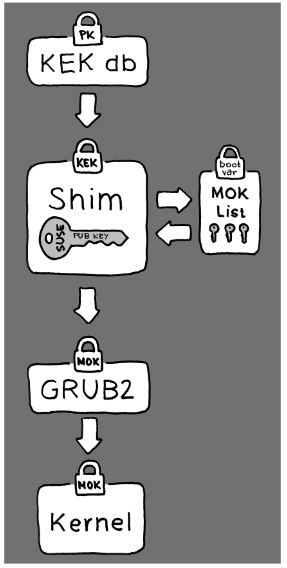
\includegraphics[scale=0.8]{img/secureboot.png}
\end{wrapfigure}
\paragraph{Secure Boot}\\
Questa tecnica si appoggia a UEFI, un sistema software piu' ampio e complesso pensato per sostituire interamente il BIOS tradizionale, che utilizza il minimo indispensabile, ovvero delle chiavi crittografiche utilizzate come elemento di verifica dell'integrita' e dell'autenticita' depositate nel firmware. Ovvero una parte fisica della memoria del sistema resa accessibili soltanto attraverso una procedura accuratamente controllata. UEFI nasce per sostituire completamente l'interfaccia fra sistema operativo e firmware, e' una specia di ``mini" sistema operativo che permtte di gestire i dischi in maniera enormemente piu' flessibile, e contiene un suo filesystem dedicato in cui conservare i bootloader. Questo fa delle verifiche a priori, ovvero impedisce materialmente ogni singolo step di boot se quello corrente non ha superato un controllo di autenticita' e integrita'. Si basa sul fatto che sul sistema sia installata una \textbf{Platform Key}, ovvero una chiave crittografica che permette di verifica se esiste sul sitema un piccolo componente, una sorta di bootloader di livello precedente a quello sopra descritto, verificato dall'hardware del BIOS utilizzando la platfom key. Questo standard e' stato sviluppato in collaborazione con Microsoft, che inizialmente era l'unica azienda a possedere le effettive chiavi,e quindi solo Microsoft poteva attestare l'autenticita' e quindi l'affidabilita' dei bootloader e dei sistemi operativi in maniera che venissero riconosciuti da \textbf{shim}. Questo avrebbe reso impossibile installare qualsiasi tipo di sistema operativo, che non fosse deciso da Microsoft, su qualsiasi sitema che adottava UEFI. 
Chiaramente cio' scateno' una quantita' di poliche non indifferenti a tal punto che Microsoft rispose immediatamente che non intendeva utilizzare questo meccanismo per limitare la liberta' degli utenti, e creo' un set di chiavi regalando alcune di queste ad altri produttori tra cui una alla Linux Foundation , un'ente no-profit che si occupa dell'ambiente Linux, con cui poter firmare i boot loader e le distribuzioni , cosi' che sia possibile utilizzare in armonia con EUFI. Ovviamente tutti i componenti, come abbiamo detto devono essere firmati, se intendo quindi modificare una parte del kernel, o di un qualsiasi altro componente dovro' poi crearne un'attestato (firma) sotto la mia responsabilita' valido solo per il mio sistema, che ne rappresenti l'autorizzazione per shim. 
\\
A tal scopo, esiste una gerarchia di chiavi, per cui io posso generarmi una chiave personale nota come \textbf{MOC, \emph{Machine Owner Key}} e con questa apporre un sigillo di autenticita' al software che intendo installare. A questo punto devo rendere riconoscibile la chiave, se intendo utilizzarla per validare l'autenticita' di un determinato componente, comunicandola a shim, e cio' e' possibile farlo in fase di pre-configurazione; sara' poi necessario un reboot ed un accesso fisico al terminale per autorizzare l'\emph{endowment}, ovvero il deposito effettivo della mia MOC all'interno della lista di MOC autorizzate. Si noti che si, questo database di chiavi puo' essere alterato, ma non a runtime e quindi da un eventuale software malevolo che va ad iniettare codice alterando il sistema di verifica perche' cio' necessita come detto un accesso fisico alla macchina.


\subsection{Hardening di secondo livello}
Visto le modalita' per un corretto avvio del sistema, comprese quelle piu attuali per garantire crittograficamente l'autenticita' e l'integrita' del boot loader e del sistema operativo , passiamo ad un secondo livello di ``\textbf{\emph{hardening}}" , ovvero il processo di messa in sicurezza e irrobustimento del sistema. Una volta appurata l'integrita' del sistema operativo, e' necessario configurarlo correttamente per far si' che l'\textbf{accesso alle risorse} segua il principio di \emph{\underline{minimo privilegio}} e il principio di \emph{\underline{negazione a priori}} di qualsiasi azione non esplicitamente autorizzata.

\subsubsection{Accesso alle risorse}
L'accesso alle risorse viene mediato dal sistema operativo; tutti i sistemi di accesso alle ricorse seguono una catena composta da 4 fasi:
\begin{itemize}
	\item \textbf{Identificazione}
	\item \textbf{Autenticazione}
	\item \textbf{Autorizzazione}
	\item \textbf{Auditing}
\end{itemize}

Dove l'\textbf{identificazione} permette di determinare quale e' il soggetto che richiede l'accesso. Normalmente questa fase viene incorporata con la fase successiva, ovvero quella di \textbf{autenticazione}, anche se in realta' le due fasi sono logicamente distinte: alcuni sistemi senza particolari esigenze di sicurezza posso funzionare benissimo basandosi su una semplice identificazione per consentire l'accesso a determinate risorse. Formalmente, l'\emph{identificazione} consente di capire qual sia il soggetto richiedende l'accesso, mentre l'\emph{autenticazione} mi permette di verificare se l'attestazione fatta dal soggetto sulla propria identita' sia veriteria o meno. Una volta confermata l'identita' del soggetto, entra in gioco la fase di \textbf{Autorizzazione}: vado a determinare se questo puo' o no puo' eseguire determinate azioni sulle varie risorse messe a disposizione dal sistema (\emph{file, device, dispositivi fisici, interfacce di rete, etc}). 
Infine, la fase di \textbf{Auditing}. Questa dal punto di vista preditivo, non ha grande valenza: se infatti voglio implementare una \emph{policy preditiva}, che quindi consenta l'utilizzo dell risorse solo a determinate categorie di utenti, devo agire attraverso i primi 3 step. Rappresenta pero' il processo attraverso cui vengono \emph{tracciate} tutte le attivita' rilevanti o eventuali tentativi di svolgere determinate azioni da parte degli utenti (\emph{tentativi di autenticazione, esecuzione di operazioni di sistema, etc}) sulle risorse del sistema. Risulta particolarmente utile sia per controllare se vengono svolte attivita' illecite o sospette e quindi monitoraggio, sia per fare forensic post-illecito, ovvero consente di avere una traccia da analizzare attraverso la quale determinare quale delle decisioni progettuali o delle implementazioni fatte presentasse un'eventuale falla logica, consentendo quindi un'operazione non corretta.

\subsubsection{Autenticazione}
L'identificazione consiste semplicemente nel presentare qualche credenziale che puo' essere uno username o una caratteristica biometrica. Per quanto riguarda invece l'autenticazione, il soggetto richiedente, deve poter presentare un \textbf{dato non falsificabile} che viene con certezza associato alla sua identita' dal verificatore, che normalmente e' il sistema operativo. 
Il dato certo che ricerchiamo puo' assumere diverse forme:

\begin{itemize}
	\item ``\emph{Qualcosa che si e'}" \\
		conferma dell'identita' per confronto di una caratteristica intrinseca della persona, quindi fisiologica o comportamentale con un dato ``biometrico" di riferimento. Spesso nei sistemi biometrici (es. \emph{smartphone, sistema di unlock-door aziendale}), la fase di identificazione e autenticazione vengono collassate all'interno di un'unico step. Si pensi all'impronte digitale, questo puo' risultare in un eventuale problema di sicurezza in particolare in sistemi estesi, in quanto non solo deve capire se l'impronta presentata e' un'impronta corretta, ma deve farlo a fronte di un numero variabile e arbitrariamente alto di impronte pre-registrate con cui confrontarla. Questo porta, per un eventuale attaccante, ad un aumento della probabilita' che presentando la propria impronta, questa venga confusa con almeno una fra quelle autorizzate, di fatto creando una situazione molto piu' favorevole paragonata ad un contesto in cui indentificazione e autorizzazione sono invece separate, dato che se dichiaro in primis una determinata identita', e poi cerco di autenticarla, avro' un solo possibile campione, con cui confrontare quello che tento di inserire diminuendo drasticamente la possibilita' di falsi positivi. Un'altra problematica legata ai dati biometrici e' che questi sono, per loro natura, soggetti ad un alto livello di ``\emph{rumore}" per cui un margine di errore deve essere per forza tenuto in considerazione , altrimenti all'opposto rischio di generare una grande quantita' di falsi negativi, ovvero di rifiuti di autenticazione a fronte di dati biometrici corretti.

	\item ``\emph{Qualcosa che si ha}"\\
		e' il processo di conferma dell'identita' attraverso il possesso di un oggetto fisico , che deve quindi esssere custodito attentamente, riconoscibile da parte della macchina che effettua il controllo (\emph{scheda a banda magnetica, smart card, token RFID, smartphone, etc\dots})

	\item ``\emph{Qualcosa che si sa}"\\
		conferma dell'identita' dimostrando la conoscenza di un dato segreto concordato in precedenza (\emph{password, Personal Identification Number - PIN, una chiave, etc\dots}), dove il problema e' che per esser veramente affidabile dovrebbe essere effettivamente un dato ricordato a memoria e non presente su qualsiai dispositivo fisico.
\end{itemize}

\subsubsection{Gestione degli utenti}
Nessun sistema e' completo senza dei meccanismi di sicurezza. Dev'essere presente un meccanismo per proteggere i file da letture o modifiche non autorizzate. Il sistema Linux si accosta  alla metodologia di UNIX attribuendo permessi ai file, permettendo ad utenti singoli e gruppi l'accesso ai file sulla base di un insieme di permessi di sicurezza per ogni file e directory. Gli account utente sono un ingranaggio fondamentale di questo meccanismo. Ogni individuo che accede ad un sistema linux deve essere in possesso di un account utente univoco. I permessi che quest'ultimo avra' sui vari oggetti nel sistema dipenderanno dall'identita' che assume internamente al sistema.

I permessi utente vengono tracciati attraverso uno \textbf{user ID} (\emph{UID}), assegnato ad un account al momento della creazione. Questo e' un vaore numerico, univoco per ogni utente. Ad ogni modo per accedere al sistema, non viene utilizzato lo user ID, bensi' un \textbf{login name}: una stringa alfanumerica di 8 o meno caratteri che l'utente puo' utilizzare per fare log in nel sistema (generalmente insieme ad una password associata)

Linux si appoggia a file ed utility speciali per gestire e monitorare gli account utenti all'interno del sistema.Vediamo alcuni degli elementi principali che partecipano in questo meccanismo:

\paragraph{\texttt{/etc/passwd}} Il file speciale \texttt{/etc/passwd} viene utilizzato dal sistema per controllare le corrispondenze tra \emph{login name} e \emph{UID}. Questo contiene diversi campi di informazione riguardanti tutti gli utenti presenti all'interno del sistema.

\begin{lstlisting}[language=bash,basicstyle=\ttfamily,frame=single,caption={Struttura di un file /etc/passwd},captionpos=b]
$ cat \etc\passwd
root:x:0:0::/root:/bin/bash
bin:x:1:1::/:/sbin/nologin
daemon:x:2:2::/:/sbin/nologin
mail:x:8:12::/var/spool/mail:/sbin/nologin
ftp:x:14:11::/srv/ftp:/sbin/nologin
http:x:33:33::/srv/http:/sbin/nologin
nobody:x:65534:65534:Nobody:/:/sbin/nologin
dbus:x:81:81:System Message Bus:/:/sbin/nologin
elliot:x:1001:1001:Elliot:/home/elliot:/bin/bash
\end{lstlisting}

I campi del file \texttt{/etc/passwd}\texttt{(-rw-r--r-- 1 root root)} contengono le seguenti informazioni:
\begin{center}
	\texttt{<Login Username>:<password>:<UID>:<GID>:<Description>:<HOME>:<Default Shell>}
\end{center}

\paragraph{\texttt{/etc/shadow}}
Il campo della \emph{password} viene settato ad \texttt{x}, per comunicare al sistema operativo che la password dell'utente relativo si trova in un'altra locazione specifica. Storicamente, questo campo conteneva la versione `hashed' della password utente. Cio' si e' rivelato poi essere un problema di sicurezza in quanto svariati programmi necessitavano l'accesso al file \texttt{/etc/passwd} per ottenere informazioni sugli utenti. Per questo motivo si e' reso necessario a rivedere questa policy. La soluzione adottata e' stata quella di spostare la password in un file separato: \texttt{/etc/shadow} accessibile solo a utenti e programmi con privilegi speciali (\emph{programma di login, passwd, etc\dots}).

\begin{lstlisting}[language=bash,basicstyle=\ttfamily,frame=single,caption={Struttura di un file /etc/shadow},captionpos=b]
$ sudo cat \etc\shadow
elliot:\$1\$d/asfAHOADqe2kjq2eLQ@LOI:11627:0:99999:7:::
\end{lstlisting}

I campi del file \texttt{/etc/shadow}\texttt{(-rw------ 1 root root)} contengono le seguenti informazioni:
\begin{itemize}
	\item \texttt{<Login Username>}
	\item \texttt{<Encrypted password>}
	\item Days since January 1, 1970, tha the password was last changed
	\item Minimum number of days before the password can be changed
	\item Number of days before the password must be changed
	\item Number of days before password expiration that the user is warned to change the password
	\item Number of days after password expires before the account will be disabled
	\item The date (stored as days since January 1, 1970) since the user account was disabled
	\item Field reserved for future use.
\end{itemize}

Grazie all'utilizzo di questo sistema si riesce ad avere un controllo molto piu' accurato sulle password degli utenti. Si puo' controllare ogni quanto un utente debba cambiare la propria password e dopo quanto tempo disabilitare l'account relativo nel caso in cui cio' non venga fatto.


\paragraph{Account di sistema e Super User}
L'utente \textbf{root} (\emph{Super User}) viene considerato il super utente, ovvero l'amministratore del sistema. Caratteristiche di questo utente sono \textbf{UID} \textbf{0} e la prorieta' di avere \textbf{privilegi illimitati}. Esistono due modi alternativi al login diretto per ottenere i privilegi di root:\\\\
\begin{tabular}{lp{12cm}}
	\texttt{su} (switch user) & Consente di passare ad un utente specificato. Lasciano non specificato il campo utente o utilizzando l'opzione '\texttt{-} permette di loggare come root. \\
	\texttt{sudo} (super user do) & Consente di eseguire un singolo comando con privilegi di root. \\\\
\end{tabular}
Come e' possibile notare, il sistema linux crea diversi account utenti adibiti a svariate funzioni. Questi non sono in realta' utenti effettivi ma prendono il nome di  \textbf{account di sistema}. Questi sono account speciali utilizzati dai servizi in esecuzione sul sistema per ottenere l'accesso alle risorse. Tutti i servizi che vengono eseguiti in background mode necessitano di essere loggati al sistema linux utilizzando uno di questi account.

Linux riserva gli UID sotto il 500 per gli account di sistema. Inoltre, alcuni servizi necessitano UID specifici per funzionare correttamente. Quando vengono creati account per utenti regolari, la maggior parte dei sistemi Linux assegnano i primi UID disponibili a partire dal 500. 

\paragraph{Gruppi}
Gli account sono efficaci per controllare la sicurezza del singolo utente, ma poco funzionali per consentire a gruppi di utenti di condividere determinate risorse. Per ottenere cio', Linux si avvale di un altro concetto di sicurezza: i \textbf{gruppi}. Notare che un utente \textbf{deve} sempre appartenere ad almeno un gruppo; normalmente il sistema, all'atto della creazione dell'utente , ne crea uno omonimo contenente solo l'utente in questione. Questi consentono a piu' utenti di condividere un insieme comune di permessi relativi ad un oggetto nel sistema, come un file, una directory o un device. Ogni gruppo ha un GID univoco, anche questo consiste di un valore numerico. Proprio come per gli account utenti, le informazioni sui gruppi sono salvate in un file di sistema: \texttt{/etc/group}. Questo contiene informazioni relative ad ogni gruppo sul sistema.

\begin{lstlisting}[language=bash,basicstyle=\ttfamily,frame=single,caption={Struttura di un file /etc/group},captionpos=b]
$ cat \etc\group
root:x:0:root
bin:x:1:root,bin,daemon
daemon,bin,daemon
sys:x:3:root,bin,adm
adm:x:4:root,adm,daemon
elliot:x:500:
mysql:x:27:
\end{lstlisting}

I campi del file \texttt{/etc/group}\texttt{(-rw-r--r-- 1 root root)} contengono le seguenti informazioni:
\begin{itemize}
	\item \texttt{<Group Name>}
	\item \texttt{<Group Password>}
	\item \texttt{<Group ID>}
	\item The list of user accounts that belong to the group
\end{itemize}
Cosi' come per gli UID, i Group ID vengono assegnati usando un formato speciale. I gruppi utilizzati per account di sistema sono assegnati GID inferiori a 500, e ai gruppi utenti vengono assegnati GID a partire dal 500.

\paragraph{Tools}
Gli utenti e i gruppi possono essere manipolati utilizzando i seguenti comandi: 

\begin{center}
\begin{tabular}{ll}
	\textbf{Account Modification Utilities} & \\
	\texttt{useradd <username>} & Creazione di un utente\\ 
	\texttt{userdel <username>} & Rimozione di un utente\\ 
	\texttt{usermod <username>} & Modifica di un utente\\ 
	\texttt{passwd <username>} & Modifica la password di un utente - Lock/Unlock dell'account\\ 
	\texttt{chsh -s <Shell Path> <username>} & Cambia la shell di default di un utente\\ 
	\texttt{chage}  & Modifica il periodo di validita' temporale di una password \\ 
	\\
	\textbf{Group Modification Utilities} & \\
	\texttt{groupadd <groupname>} & Creazione di un gruppo \\
	\texttt{groupmod <groupname>} & Modifica di un gruppo \\ 
	\\
\end{tabular}
\end{center}

Entrambi i comandi supportano varie opzioni consultabili attraverso le \texttt{man pages}.

\begin{center}
	\begin{tabular}{lp{10cm}}
	\textbf{Identita' e Utenti} & \\
	\texttt{whoami} & Riporta il proprio username \\
	\texttt{id <username>} & Fornisce una serie di informazioni sull'identita' e sul gruppo di appartenenza dell'utente\\
	\texttt{who} & Indica quali utenti sono attualmente connessi al sistema\\
	\texttt{last} & Elenca uno storico dei collegamenti \\
	\end{tabular}
\end{center}


\subsubsection{Password}
La scelta di una password, dovrebbe essere una scelta dettata da ragioni scientifiche. Questa deve possedere due caratteristiche che sono in contrastro una con l'altra: deve essere memorizzabile ma al contempo impossibile al lato pratico da indovinare o da predire per chiunque non sia il proprietario dell'identita' associata. E' quindi importante scegliere accuratamente delle password che siano sufficentemente robuste da garantire la sicurezza di un sistema, questo in particolare per quelle utenze con privilegi amministrativi o comunque elevati, ma e' valido anche per le utenze regolari del sistema. Un eventuale attaccante che entrasse in possesso delle credenziali di un nostro utente, diventando quindi un \emph{insider}, si troverebbe in una situazione nettamente favorevole per pianificare eventuali azioni malevole; la consapevolezza di chi amministra il sistema non basta, e' importante educare chi utilizza il nostro sistema , e quindi i nostri utenti, a fare scelte dettate dalla consapevolezza  di chi utilizza un determinato ambiente e quindi contribuisce a tutelarne l'integrita'. Una volta accordate e decretate delle policy per la scelta delle password bisogna poi convincere gli utenti ad applicarle. Se queste sono troppo rigide, il risultato collaterale puo' essere che gli utenti comincino ad utilizzare altri espedienti (\emph{post-it, etc}) attaccati ovunque per essere sicuri di non dimenticarle, creando di fatto un possibile problema di sicurezza. Si puo' utilizzare un altro approccio, che e' quello \emph{reattivo}, cioe' ci si mette nei panni di un attaccante e cercando di mettere in atto un attacco volto a svelare eventuali password ovvero testarne la robustezza attraverso tool automatici (\emph{John The Ripper}) per poi allertare chi eventualmente, in buona fede o non, ha fatto scelte poco efficaci.
\paragraph{Entropia}
Un concetto che nella scelta delle password assume un ruolo fondamentale e' quello di \textbf{entropia}. Questa e' una misura della quantita' di \textbf{incertezza} o \textbf{impredicibilita}'di un eventuale informazione. Innanzitutto, per comprendere meglio questo concetto, e' importante partire dalla scienza che sta dietro la rappresentazione di un'informazione: cosa intendiamo per quantita' di informazione contenuta in un dato? L'informazione e' assimilabile alla difficolta' di prevedere quel dato. Un bit di informazione, ricevuto dall'esterno, presenta un'incertezza del 50\% (0 o 1) prima che venga ricevuto; capire quindi la quantita' di informazione significa quindi risolvere un dubbio fra le due possibili opzioni che si potrebbero presentare. L'entropia, ovvero la quantita' di informazione convogliata da una stringa, equivale quindi al numero di possibili configurazioni di quella stringa e, conseguentemente, a quanto e' ampio il `dubbio' che si intende risolvere.
\begin{figure}[H]
	\centering
	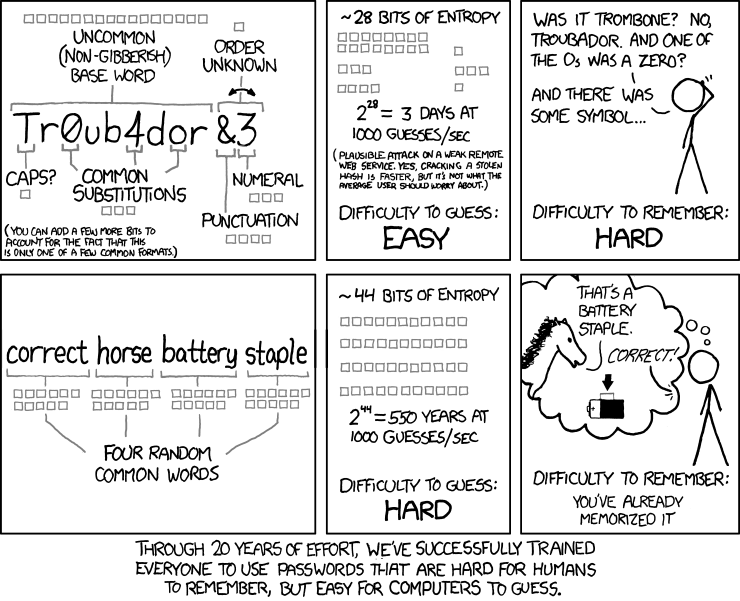
\includegraphics[scale=0.5]{img/entropiaxkcd.png}
	\caption{Password strength - \url{http://xkcd.com/936/}}\label{entropy}
\end{figure}
E' importante comprendere come non sempre l'entropia sia direttamente proporzionale alla quantita' di bit con cui viene codificata l'informazione. Prendendo , per esempio, una fra le circa 65'000 parole del dizionario inglese, ottengo una stringa che ha un'entropia pari a 65'000 possibili combinazioni , $ 2^{16} = 65'536 $, ovvero pari a 16 bit necessari a rappresentarle. Notare pero' che l'entropia di questa parola e' totalmente sconnessa rispetto al numero di bit con cui e' codificata all'interno del computer: presa una parola di 11 lettere codificata in ASCII standard 8 bit, questa occupera' uno spazio di memoria pari a $11 * 8 = 88$ bit, ma il fatto che io abbia bisogno di renderla memorizzabile, e che quindi sia un vera parola del dizionario della lingua inglese, fa si che l'entropia effettiva sia 16 e non 88, in quanto corrisponde alla difficolta' di indovinarla fra una delle circa 65'000 parole del dizionario e non quella di trovare la configurazione di 88 bit con cui quella stringa e' codificata in ASCII. Questo e' un punto fondamentale in quanto puo' creare una falsa sensazione di sicurezza.
\begin{center}
	\emph{Ma quanta entropia aggiungono tutte le modifiche che posso eventualmente apportare ad una stringa?}
\end{center}
\paragraph{Figura \ref{entropy}}
La prima lettera la metto in maiuscolo oppure no? Questa domanda si muove in uno spazio binario di possibili scelte (\emph{si, no}), aggiungeno di fatto un bit effettivo di entropia. Se trasformassi le eventuali vocali, nei corrispettivi numeri in base alla somiglianza grafica (le O in 0, le A in 4, etc..), allo stesso modo introdurrei un bit di entropia, in quanto l'incertezza sta nel capire se ho o meno adottato questo tipo di trasformazione. Posso pensare di appendere alla fine della stringa dei caratteri di punteggiatura o dei numeri, in che ordine? Stessa tipologia di incertezza, introduco un bit di entropia. Il numero? sono 3 o 4 bit. Il carattere di punteggiatura? Una dozzina di bit tra cui scegliere. Una volta portate alla luce tutte queste fonti di incertezza , e' possibile fare la somma ottenendo 28 bit di entropia effettivi. Su un calcolatore in grado di fare \texttt{1000 tenativi/sec} , la password viene crackata in un tempo massimo di 3 giorni.
Abbiamo almeno ottenuto una password facile da ricordare? Se abbiamo aperto il dizionario e scelto una parola a caso probabilmente non sara' una parola molto significativa per noi, e quindi facile da ricordare. Puo' essere che l'introduzione di tutta questa casualita' vada poi a ritorcersi contro l'utente stesso che deve memorizzarla, o comunque avere a mente uno schema preciso per ottenerla. 

\paragraph{Passphrase}
Un'alternativa valida e' quella di utilizzare delle \emph{passphrase}. Queste presentano l'innegabile svantaggio di essere particolarmente lunghe perche' vanno a fare un compromesso diverso: si basano infatti sull'idea di scegliere un numero $N$ di parole di uso estremamente comune (o non) per accumulare tanti contributi di entropia piu' ridotti finche' non si mettono insieme abbastanza bit da rendere la password piu' sicura. Nella seconda parte della vignetta in Figura \ref{entropy}, viene riproposta riproposta la stessa analisi pertendo pero' da 4 parole casuali non all'interno dell'intero dizionario della lingua inglese, che contiene circa 65'000 vocaboli, ma all'interno del dizionario ridotto delle circa 2000 parole che vengono comunemente usate nel linguaggio di tutti i giorni, ovvero parole con un'altissima probabilita' di essere facili da ricordare e anche piu' facilmente inseribili in una frase attraverso qualche tecnica di visualizzazione. Riprendendo quindi l'esempio, abbiamo ottenuto una passphrase facile da ricordare, che al contempo potrebbe pero' sembrare meno sicura in quanto composta da parole `semplici'; Andando ad analizzarla, se ogni parola e' scelta fra le 2000 parole piu' comuni, la sua entropia sara' ridotta a $2^{11} = 2048$ bit. Avendone pero' scelte 4, il totale di entropia della frase e' $2^{11x4} = 2^{44} \approx 1.7 \times 10^{13}$; essendo che la valutazione segue una legge esponenziale, cio' significherebbe , a parita' di potenza di calcolo con la macchina presa in considerazione prima, passare da 3 giorni a 550 anni in tempo di calcolo.

\paragraph{Password Manager}
Questo discorso puo' risultare particolarmente difficile da applicare quando ci si trova a dover gestire e quindi memorizzare le password di diverse decine se non centinaia di account; anche a fronte del fatto che per evitare attacchi di tipo cross platform, sarebbe opportuno che le password impiegate fossero tutte differenti. A tal proposito, per adempire a queste necessita' sono stati sviluppati svariati sistemi di password management, in cui e' possibile archiviare in modo sicuro e cifrato tutte le password che si dispongono, per poi proteggere l'intero sistema con un'unica chiave robusta, che a questo punto potra' essere una passphrase accuratamente costruita.

\paragraph{Eta' delle password}
Come abbiamo visto il tempo e' un fattore chiave, nell'ottica in cui cerchiamo di costruire password in maniera tale che siano non impossibili da trovare, ma la cui ricerca si muova in uno spazio talmente ampio di possibilita' da risultare impossibile da trovare con una quantita' di risorse plausibili e in un tempo utile ai nostri fini. Un'ulteriore contromisura e' quindi data dall'evitare che una password possa rimanere la stessa per periodi di tempo troppo lunghi.

\paragraph{Password in Linux}
Quando si esegue un login o si imposta una password ad un utente del sistema, questa viene processata attraverso una funzione \textbf{one-way hash}, e salvata o confrontata con quella gia' presente all'interno del file \texttt{/etc/shadow}, cosi' da non avere mai la necessita' di mantenere informazioni sensibili in chiaro a disposizione di un eventuale attaccante che dovesse impossessarsene. La robustezza di questo meccanismo e' garantito da una caratteristica fondamentale delle funzioni hash, ovvero quella di essere non invertibili, rendendo quindi il processo di ricerca della password originale molto piu' complesso: richiede infatti che vengano provate tutte le possibili combinazioni di password plausibili , passate attraverso la medesima funzione hash (pubblicamente nota) e confrontate con il valore hash di cui si intende determinare l'origine. Piu' formalmente la funzione hash e' una funzione che mappa infiniti possibili input in un numero finito di output , producendo infatti stringhe di dimensione finita e fissa; questo ci dice che idealmente esistono infinite password che potrebbero avere lo stesso hash. Quindi bisogna accuratamente valutare la grandezza del codominio, in quanto puo' anche darsi che l'attaccante trovi una password diversa dalla nostra ma che al contempo produca lo stesso hash, motivo per cui una delle proprieta' che si ricerca in queste funzioni e' la \emph{collision-freedom}, ovvero una bassissima probabilita' che due elementi del dominio, possano produrre lo stesso elemento del codominio.

\paragraph{Policy}
I sistemi UNIX, inoltre, implementano vari meccanismi , anche attraverso le librerie di gestione delle credenziali, che permettono non solo di stabilire dei criteri di complessita' ma anche di stabilire dei criteri di riuso. Ad esempio configurando il modulo \textbf{PAM} (\emph{Pluggable Authentication Module}).

\subsubsection{Autorizzazione}
Vediamo ora cosa significa limitare l'uso dell risorse da parte di utenti che si siano correttamente autenticati e collegati al sistema. 

\paragraph{Limits}
Partiamo da un tipo di autorizzazione generale, che \emph{limita} l'uso delle risorse pirncipalmente per evitare che il sistema possa essere monopolizzato da un utente a discapito della disponibilita' di quelle stesse risorse verso gli altri utenti. Questo e' il sistema dei \textbf{limits}. In un quadro di sicurezza, questi possono essere impiegati per far fronte e limitare eventuali attacchi di tipo \emph{Denial of Service}, ma possono fungere anche da salvaguardia contro gli incidenti interni. Questi limiti possono essere configurati localmente alle shell che vengono lanciate attraverso il comando \texttt{ulimit} e possono essere configurate centralmente con il modulo del sottosistema che si occoupa di autenticazione \texttt{pam\_limit} configurato attraverso il file \texttt{/etc/limits.conf}; in questo file sono presenti record nella forma:
\begin{center}
	\texttt{<domain> <type> <item> <value>}
\end{center}
\begin{tabular}{lp{12cm}}
	\texttt{<Domain>} & \texttt{user, @group, *} \\
	\texttt{<Type>} & \texttt{hard, soft, -} (both). Un limite \emph{hard} viene imposto da root come valore massimo, e non puo' essere superato dall'utente,mentre un limite \emph{soft} e' un valore di default modificabile dall'utente entro il massimo permesso dal S.O e dal limite hard.\\ 
	\texttt{<Item>} & Rappresentano le risorse alle quali e' possibile applicare questi limiti (Figura \ref{limitstype})
\end{tabular} 
\begin{figure}[H]
	\centering
	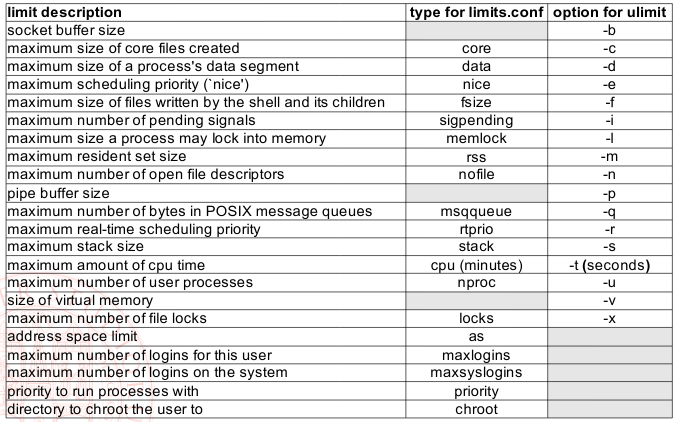
\includegraphics[scale=0.8]{img/typelimits.png}
	\caption{Tipologie di item per i limits}\label{limitstype}
\end{figure}

\subsubsection{Modelli di controllo dell'accesso}
Se il discorso dei limits si applica spesso a tipologie di risorse shared fra gli utenti di sistema (\emph{ram, cpu, dischi, etc..}), i modelli di controllo dell'accesso si focalizzano su risorse non necessariamente condivise ma che possono essere presenti in moltissime istanze sul sistema in un numero variabile e dinamicamente modificabile, applicando un controllo piu' puntuale. Ogni qualvolta sul sistema vado a creare un file posso `etichettarlo' in modo tale che un sottoinsieme specifico di utenti possano svolgere un sottoinsieme specifico di operazioni su quella risorsa. 
\begin{center}
	Parlando in termini generali, il sistema di controllo dell'accesso e' idealmente una matrice che permette di decidere se un \textbf{soggetto} (entita' attiva che vuole fare delle operazioni) puo' eseguire una specifica \textbf{operazione} su di un \textbf{oggetto}, ovver la risorsa su cui il soggeto vuole operare.
\end{center}
I soggetti sono entita' attive quali \emph{utenti, gruppi di utenti, processi}. Gli oggetti sono qualunque risorsa sia disponibile sul sistema (\emph{file, directory, socket di rete, o anche altri processi}). 
Idealmente, la politica di controllo dell'accesso puo' essere rappresentata come una matrice che all'incrocio tra ogni possibile soggetto e ogni possibile oggetto ha l'elenco dei permessi. Questo tipo di rappresentazione e' pero poco scalabile a sistemi estesi,in cui possono esserci migliaia di utenti e milioni di oggetti, diventando di fatto ingestibile. Sorge quindi un'osservazione: tutte queste celle contengono effettivamente informazioni uniche e non rappresentabili? La risposta e' no. Nella maggior parte dei casi, infatti, queste celle contengono dei valori di default, non e' quindi necessario specificare esplicitamente su ogni singola risorsa quali siano i permessi associati ad ogni singolo utente in quanto , normalmente anche a fronte del principio di minimo privilegio, il set di permessi standard e' minimo e posso limitarmi ad elencare solo le eccezzioni alla regola, ovvero chi esattamente puo' fare qualcosa su quella risorsa. \\
Fatta questa osservazione, e' possibile notare come in una tabella generica, la maggior parte delle celle sia vuota, il che equivale a dire che contiene un valore di default predicibile e che quindi posso comprimerla, utilizzando due metodologie diverse:
\begin{itemize}
	\item \textbf{Capability List} \\
		Partizionare la matrice dell'accesso colonna per colonna, ovvero per soggetto; il che vuol dire  associare ad ogni utente, una lista di permessi, nota come \textbf{capability list}, contenente tutte le capacita', diverse da quelli di default, che l'utente possiede sulle varie risorse di sistema. Questa soluzione non viene adottata dai sistemi comuni, bensi' da sistemi piu' complessi che adottano una policy centralizzata di controllo degli accessi nota come \textbf{MAC}(\emph{Mandatory Access Control}). In questo modello, oltre all'utilizzo delle capability list, esiste anche il concetto di controllo dell'accesso forzato: un utente eletto a `security manager', scrive questa serie di capability list in un file di configurazione e nessuno ha piu' il diritto di modificarle.
	\item \textbf{Access Control List}\\
		Ortogonalmente, potrei decidere di partizionare la matrice per righe (o per oggetti); ovvero associare ad ogni file una lista di utenti e relativi permessi, diversi da quelli di default, che possono esercitare sull'oggetto in questione. Questo meccanismo e' quello piu' comunemente utilizzato anche da POSIX (lo standard che riunisce tutti gli standard di UNIX e Windows nel sistema NTFS) nei sistemi che adottano una policy decentralizzata del tipo \textbf{DAC} (\emph{Discretionary Access Control}), ovvero controllo dell'accesso a discrezione. Cio' significa che ogni oggetto ha un proprietario che tipicamente e' il soggetto creatore, e la discrezione si realizza nella possibilita' da parte del proprietario di modificare l'ACL di quell'oggetto a propria discrezione. Nel filesystem UNIX il modello delle ACL e' ulteriormente semplificato in quanto non esistono delle liste generiche; ogni file viene descritto attraverso un inode all'interno di questa struttura dati e' contenuta viene memorizzato esattamente un utente e un gruppo proprietario del file accompagnato da un set di 12 bit che rappresentano i permessi standard e quelli speciali. Avremo quindi un ACL standard composta di fatto da 3 campi.
\end{itemize}
\begin{figure}[H]
	\centering
	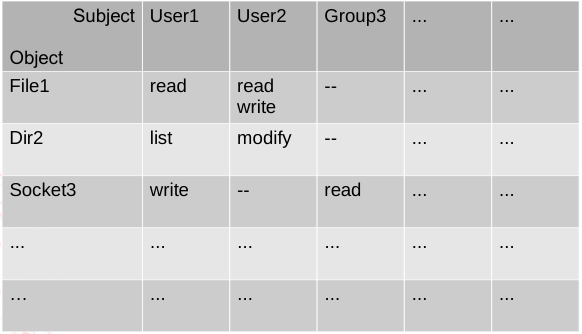
\includegraphics[scale=0.5]{img/acmatrix.png}
	\caption{Matrice per il controllo dell'accesso}
\end{figure}

\subsubsection{Proprieta' dei file e permessi}
Sotto il modello tradizionale dei filesystem UNIX e Linux, ogni file possiede un set di 9 bit di permessi con lo scopo di controllare chi puo' leggere, scrivere ed eserguirne il contenuto. Insieme ad altri 3 bit che interessano principalmente le operazioni dei file eseguibli, questi bit constituiscono il `\emph{modo}' del file.

\begin{lstlisting}[language=bash,basicstyle=\ttfamily,frame=single,caption={Output del comando \texttt{ls -l}},captionpos=b]
-rw-r--r-- 1 damn users  3874 Mar 18 18:25 Approfondimenti.tex
-rw-r--r-- 1 damn users 15152 Mar 18 18:25 Command-line.tex
drwxr-xr-x 2 damn users  4096 Mar 19 21:18 img
-rw-r--r-- 1 damn users   252 Mar 18 19:22 Makefile
-rw-r--r-- 1 damn users   729 Mar 18 18:25 Master.tex
\end{lstlisting}
Il primo campo nell'output del comando listing e' un codice che rappresenta i permessi per i file e le directory. In linux i file si articolano in varie tipologie; il primo carattere nel campo dei permessi stabilisce il \textbf{tipo} dell'oggetto:
\begin{itemize}
	\item \texttt{-} Regular files 
	\item \texttt{d} Directories 
	\item \texttt{l} Links 
	\item \texttt{c} Character Device 
	\item \texttt{b} Block Device 
	\item \texttt{n} Network Device 
\end{itemize}
Dopo questo, si possono distinguere 3 set composti da 3 caratteri ciascuno. Ognuno di questi set di tre caratteri definisce una \textbf{tripletta di permessi}:
\begin{itemize}
	\item \texttt{r} Read (Lettura del contenuto)
	\item \texttt{w} Write (Modifica del contenuto)
	\item \texttt{x} Execute 
\end{itemize}
\noindent\rule{16cm}{0.4pt}\\
Alcune \textbf{precisazioni}:
\begin{itemize}
	\item Il permesso \texttt{w} Write consente ad un utente di cancellare all'interno di una directory, indipendentemente dai permessi che questo ha sugli specifici file al suo interno.
	\item Per una directory, il bit \texttt{x} execute (spesso chiamato bit di `ricerca' o `scan' in questo contesto) permette alla directory di essere acceduta o attraversata durante la risoluzione di un pathname, ma non permette di mostrarne il contenuto. La combinazione dei bit di read ed execute permette di mostrare il contenuto di una directory. La combinazione dei bit di write ed execute permette di creare, cancellare e rinominare file all'interno della directory.
	\item Un utente puo' rientrare all'interno di 2 categorie di permessi. Si noti che un comportamento assolutamente deterministico messo in atto dai sistemi UNIX e' quello di applicare i permessi relativi alla prima categoria di appartenenza del soggetto (ovvero i piu' specifici) nel percorso `Permessi Utente' $\rightarrow$ `Permessi Gruppo' $\rightarrow$ `Permessi Altri'.  
\end{itemize}
\noindent\rule{16cm}{0.4pt}\\
Se uno o piu' specifici permessi vengono negati, il carattere \emph{dash} (\texttt{-}) comparira' nelle corrispondenti posizioni all'interno della tripletta. I tre insiemi di caratteri rappresentano 3 livelli di sicurezza per l'oggetto:
\begin{itemize}
	\item Il proprietario (\texttt{Owner}) dell'oggetto
	\item Il gruppo di appartenenza (\texttt{Group}) dell'oggetto
	\item Chiunque altro all'interno del sistema (\texttt{Others})
\end{itemize}
\begin{table}[]
\centering
\begin{tabular}{cccc}
\hline
\rowcolor[HTML]{C0C0C0} 
\multicolumn{1}{c|}{\cellcolor[HTML]{C0C0C0}\textbf{Permissions}} &
\multicolumn{1}{c|}{\cellcolor[HTML]{C0C0C0}\textbf{Binary}} &
\multicolumn{1}{c|}{\cellcolor[HTML]{C0C0C0}\textbf{Octal}} &
\multicolumn{1}{c}{\cellcolor[HTML]{C0C0C0}\textbf{Description}} \\ \hline
--- & 000 & 0 & No \emph{permission}                      \\ \hline
--x & 001 & 1 & Execute-only \emph{permission}            \\ \hline
-w- & 010 & 2 & Write-only \emph{permission}              \\ \hline
-wx & 011 & 3 & Write and Execute \emph{permission}       \\ \hline
r-- & 100 & 4 & Read-only \emph{permission}               \\ \hline
r-x & 101 & 5 & Read and Execute \emph{permission}        \\ \hline
rw- & 110 & 6 & Read and Write \emph{permission}          \\ \hline
rwx & 111 & 7 & Read, Write and Execute \emph{permission} \\ \hline
\end{tabular}
\caption{Linux File Permission Codes}
\end{table}
I tre gruppi (o livelli di sicurezza) definiscono i permessi sull'oggetto rispettando il seguente ordine.
\begin{center}
	\texttt{<Owner Permission><Group Permission><Everyone else Permission>}
\end{center}
Risulta conveniente discutere i permessi in termini di numeri ottali (base 8) poiche' ogni cifra di un numero ottale rappresenta 3 bit e ogni gruppo di permessi consiste di 3 bit.

\paragraph{umask}
Ogni volta che creiamo un file questo assume un set di permessi di default. Il comando \texttt{umask} permette di determinare la configurazione di una `maschera' (\textbf{file mode creation mask}) che ha lo scopo di filtrare i set di permessi per i file creati. Influisce inoltre sui permessi che vengono modificati esplicitamente. Per maschera si intende un insieme di bit, ognuno dei quali limita il corrispondente permesso di default impostato per i file creati ex-novo. Permette quindi di `mascherare' quei permessi che non vogliamo attribuire ad un determinato livello di sicurezza. Cio' viene fatto sottraendo la maschera dall'insieme totale dei permessi di default attribuiti ad un oggetto: nel caso dei file questi corrispondono a \texttt{666} (Read/Write per tutti i livelli), mentre per le directory a \texttt{777} (Read/Write/Execute per tutti i livelli).
\begin{lstlisting}[language=bash,basicstyle=\ttfamily,frame=single,caption={Calcolo dei permessi},captionpos=b]
Standard file permission: 	OCTAL		BINARY
Read-Write			666		110 110 110
Mask Applied:			022		000 010 010
	
					Perm.	110 110 110 &
					!Mask	111 101 101 =
					---------------------
Resulting Permission:		644		110 100 100
\end{lstlisting}
Il valore di default della \texttt{umask} viene generalmente impostato nello start-up file \texttt{/etc/profile} (letto dalla shell), oppure nel file \texttt{/etc/login.def} (Ubuntu). All'interno di una sessione di shell e' comunque possibile specificare valori di umask diversi da quella di default attravero il comando \texttt{umask}.
\paragraph{Bit speciali}
Ci sono 3 bit di informazione addizionali che Linux mantiene per ogni file e directory:
\begin{itemize}
	\item \textbf{Set user id (SUID)}\\
		Quando un file viene eseguito da un utente, il programma `gira' con i privilegi dell'utente proprietario.
	\item \textbf{Set group id (SGID)}\\
		Per un file, il programma viene eseguito con i permessi del gruppo proprietario del file. Per una directory, tutti i nuovi file creati all'interno di questa utilizzano il gruppo della directory come gruppo di default. Questo bit e' importante in particolare per la condivisione di file. Una volta abilitato, e' possibile `forzare' i permessi di tutti i nuovi file creati in una directory condivisa , in modo che questi siano sotto il possesso del gruppo della directory. Il SGID bit puo' essere impostato attraverso il comando \texttt{chmod} (Sezione \ref{chmodchown}).
	\item \textbf{Sticky bit}\\
		Se viene settato su un file regolare (obsoleto), questo rimane (`sticks') in memeoria anche dopo la fine del processo. Se settato su una directory, invece, il filestystem non permettera' a nessuno che non sia o il proprietario della cartella, o il proprietario del file, o root di cancellare o rinominare un file. Questa convensione contribuisce a rendere directory come \texttt{/tmp} (world-writable) piu' private e sicure, imponendo che nella directory i file siano cancellabili solo dai rispettivi proprietari.
\end{itemize}
SUID e SGID sono un modo efficace per implementare interfacce per utenti standard verso processi privilegiati. Ad esempio il cambio della password attraverso il tool \texttt{passwd}, o la pianificazione di attivita' tramite \texttt{crontab} , etc. Al contempo i programmi con questi privilegi vanno accuratamente sorvegliati, poiche' chiunque li lanci acquisisce temporaneamente privilegi potenzialmente elevati. Il comando \texttt{find} (Sezione \ref{findcmd}) fornisce uno strumento efficace a questo scopo.

\begin{table}[]
\centering
\begin{tabular}{cccc}
\hline
\rowcolor[HTML]{C0C0C0} 
\multicolumn{1}{c|}{\cellcolor[HTML]{C0C0C0}\textbf{Binary}} &
\multicolumn{1}{c|}{\cellcolor[HTML]{C0C0C0}\textbf{Octal}} &
\multicolumn{1}{c}{\cellcolor[HTML]{C0C0C0}\textbf{Description}} \\ \hline
000 & 0 & All bit are cleared.                      \\ \hline
001 & 1 & The sticky bit is set.            \\ \hline
010 & 2 & The SGID bit is set.              \\ \hline
011 & 3 & The SGID and sticky bits are set.       \\ \hline
100 & 4 & The SUID bit is set.               \\ \hline
101 & 5 & The SUID and sticky bits are set.        \\ \hline
110 & 6 & The SUID and SGID bits are set.          \\ \hline
111 & 7 & All bits are set.		\\ \hline
\end{tabular}
\caption{Linux File Permission Codes}
\end{table}

\subsubsection{Modificare proprieta' e permessi dei file}\label{chmodchown}
Linux mette a disposizione diverse utilities per modificare le impostazioni di sicurezza di un file o una directory.

\paragraph{Modificare i permessi dei file}
Il comando \texttt{chmod} permette di cambiare le impostazioni di sicurezza per file e directory. Il formato del comando e':
\begin{center}
	\texttt{chmod <options> <mode> <file>}
\end{center}
Il parametro \textbf{mode} permette di settare le impostazioni di sicurezza utilizzato sia il formato ottale che quello symbolico. Per quello ottale basta utilizzare le 3 cifre ottali corrispondenti ai nuovi permessi che si vogliono attribuire ai vari livelli di sicurezza della risorsa. E' pero possibile utilizzare anche un altro approccio: la notazione \emph{simbolica}. Questa si conforma al seguente pattern:
\begin{center}
	\texttt{[ugoa..] [+-=] [rwxXstugo]}
\end{center}
Il primo gruppo di caratteri difinisce a chi applicare i nuovi permessi:
\begin{itemize}
	\item \texttt{u} for the user 
	\item \texttt{g} for the group
	\item \texttt{o} for the others (everyone else) 
	\item \texttt{a} for all of the above
\end{itemize}
Successivamente, viene utilizzato un simbolo per indicare l'azione da svolgere con i permessi, ovvero, se si intende aggiungere i permessi a quelli preesistenti (+), sottrarre i permesssi a quelli preesistenti (-), o settare i permessi ad uno specifico valore (=).
Infine, il terzo simbolo specifica il permesso in questione. In aggiunta a quelli gia' definiti, troviamo:
\begin{itemize}
	\item \texttt{X} assign execute permissions only if the object is a directory or if it already had execute permission. 
	\item \texttt{s} sets the UID or GID on execution.
	\item \texttt{t} saves program text.
	\item \texttt{u} sets the permissions to the owner's permissions.
	\item \texttt{g} sets the permissions to the group's permissions.
	\item \texttt{o} sets the permissions to the other's permissions.
\end{itemize}

\paragraph{Modificare la proprieta' dei file}
 Il comando \texttt{chown} e \texttt{chgrp} permette di modificare rispettivamente il proprietario e il gruppo di default di una determinata risorsa.
Il formato del comando \texttt{chown} e':
\begin{center}
	\texttt{chown <options> <owner[.group]> <file>}
\end{center}
Per cambiare il default group di un file, e' necessario essere il proprietario di questo e appartenere al gruppo che si sta tendando di settare. E' possibile utilizzare questo comando in maniera ricorsiva su una directory e i relativi file contenuti, usando l'opzione \texttt{\textbf{- R}}.

\subsubsection{Bonus flags: attributi dei file}
Linux definisce un insieme di flag supplementari che possono essere settate sui file per richiedere speciali trattamenti. Per fare cio' utilizza i comandi \texttt{lsattr} e \texttt{chattr} per mostrare e modificare gli attributi di un determinato file. La tabella \ref{fileattributes} mostra alcune delle flags piu' utilizzate.

\begin{table}[H]
\centering
\begin{tabular}[H]{ccp{13cm}}
\hline
\rowcolor[HTML]{C0C0C0} 
\multicolumn{1}{c|}{\cellcolor[HTML]{C0C0C0}\textbf{Flag}} &
\multicolumn{1}{c|}{\cellcolor[HTML]{C0C0C0}\textbf{FS^{a}}} &
\multicolumn{1}{c}{\cellcolor[HTML]{C0C0C0}\textbf{Meaning}} \\ \hline
\texttt{A}& XBE & Never update access time (\emph{st\_atime}; for performance)\\ \hline
\texttt{a}& XBE & Allow writing only in append mode (Avoid log cut)\\ \hline
\texttt{i}& XBE & Make this file immutable \\ \hline
\end{tabular}
\caption{\texttt{File's attribute}}\label{fileattributes}
\end{table}
a. X=XFS, B=Btrfs, E=ext3 and ext4

\subsubsection{Utility \textbf{find}}\label{findcmd}
Il comando \texttt{find} e' un utility efficance per la ricerca di file con determinate caratteristiche all'interno di una gerarchia di directory. Il formato di find rispetta lo schema seguente:
\begin{center}
	\texttt{find [starting-point...] [expression]}
\end{center}
GNU find ricerca all'interno di directory radicate negli starting-point valutando l'espressione data da sinistra a destra. Se non viene specificato nessun starting-point, viene considerata la directory corrente `\texttt{.}'. La parte successiva alla lista di starting-point e' l'espressione. Questa e' una sorta di specifica della query che descrive quali file rientrino nei nostri parametri di ricerca. E' possibile specificare l'espressione nella forma di `TEST' , il quale restituira un valore booleano determinando quali file o directory compariranno poi nel risultato finale della ricerca; Nella Tabella \ref{findcmdtests} sono elecati alcuni di questi. Find e' un tool potentissimo, con una quantita' innumerevole di opzioni e possibilita' consultabili tramite \texttt{man find}.
\renewcommand{\arraystretch}{1.5}
\begin{table}[H]
\centering
\begin{tabular}[H]{cp{13cm}}
\hline
\rowcolor[HTML]{C0C0C0} 
\multicolumn{1}{c|}{\cellcolor[HTML]{C0C0C0}\textbf{Test}} &
\multicolumn{1}{c}{\cellcolor[HTML]{C0C0C0}\textbf{Description}} \\ \hline
\texttt{-empty}	& File is empty and is either a regular file or directory\\ \hline
\texttt{-nouser}	& No user corresponds to file's numeric user ID\\ \hline
\texttt{-nogroup}	& No group corresponds to file's numeric group ID\\ \hline
\texttt{-executable}	& Matches files which are executable and directories which are searchable by the current user.\\ \hline
\texttt{-ctime \underline{n}}	& File's status was last changed \underline{n}*24 hours ago.\\ \hline
\texttt{-name \underline{pattern}}	& Base of file (the path with leading directories removed) name matches shell pattern \underline{pattern}.\\ \hline
\texttt{-iname \underline{pattern}}	& like \texttt{\textbf{-name}}, but the match is case insensitive.\\ \hline
\texttt{-regex \underline{pattern}}	& File name matches regular expression \texttt{\textbf{regex}}\\ \hline
\texttt{-perm \underline{mode}}	& File's permission bits are exactly \texttt{\textbf{mode}}\\ \hline
\texttt{-perm \underline{-mode}}	& All the permission bits \texttt{\textbf{mode}} are set for the file\\ \hline
\texttt{-perm \underline{/mode}}	& Any of the permission bits \texttt{\textbf{mode}} are set for the file\\ \hline
\texttt{-type \underline{c}}	& File is of type \texttt{\textbf{c}} (File's type on man page).\\ \hline
\end{tabular}
\caption{\texttt{Find's tests}}\label{findcmdtests}
\end{table}

\subsubsection{POSIX Access Control Lists}
POSIX e' rimasta fedele alla granularita' dei 3 bit \texttt{rwx} introducendo pero' dei meccanismi che permettessero di estendere la flessibilita' dei sistemi di autorizzazione: le \textbf{Access Control List} (ACL). Queste permettono di specificare una lista arbitraria di utenti e gruppi coi relativi permessi che vanno ad aggiungersi a quelli degli owner della risorsa. Cio' e' possibile attraverso i tool \texttt{setfacl} e \texttt{getfacl}. E' possibile sapere se un'ACL e' presente per un file attraverso il comando \texttt{ls -l} e verificando se sia presente un '\texttt{+} dopo la stringa di permessi. E' inoltre possibile specificare una mask che viene applicata in AND logico su tutti i permessi di chiunque , stabilendo cosi' un threshold ai permessi assegnabili ad una determinata risorsa; questo e' particolarmente utile in quanto le ACL a differenza dei permessi standard vengono ereditate, ovvero quando viene creato un file all'interno di una directory con ACL attive, queste vengono ereditate dai file. Mentre invece in UNIX normalmente non c'e' ereditarieta' dei permessi da parte dei file contenuti nella directory, i permessi dei file vengono sempre decretati dalla umask attiva in quel momento.

\subsubsection{Sfaccettature della security}
Quando si parla di sicurezza, questa identifica due tipologie di minacce completamente differenti: le minacce \emph{accidentali} (\textbf{safety}) e le minacce \emph{intenzionali} (\textbf{security}). In realta' molte delle tematiche che esistono nella letteratura tecnica e scientifica per questi due mondi, sono affini, in quanto la \emph{security} e' un sovrainsieme della \emph{safety}. Se voglio che un sistema sia veramente sicuro, devo anche accertarmi che eventi accidentali non violino la riservatezza, l'integrita' e la disponibilita' delle informazioni e dei servizi.




